\documentclass[dvipdfmx,cjk]{beamer} 
\usepackage{graphicx}
\usepackage{tikz}
\usetheme{CambridgeUS} 

\begin{document}


\title[Halide]{ステンシル計算言語Halide}
\author[T. Muranushi]{村主崇行\\special thanks: 似鳥啓吾}            %% ここに書かれた情報は色々なところに使われるので
\institute[RIKEN/AICS]{計算科学研究機構}   %% なるべく設定した方が良い

\begin{frame}                  %% \begin{frame}..\end{frame} で 1 枚のスライド
\titlepage                     %% タイトルページ
\end{frame}

\begin{frame}                  %% 目次 (必要なければ省略)
\tableofcontents
\end{frame}

\section{はじめに} 

\begin{frame}\frametitle{ステンシル計算とは?}
配列変数を更新していくタイプのアルゴリズムで、配列の各要素を、それぞれ近傍の要素の値のみに基づき、同じルールで更新
するものをいう。
\end{frame}

\begin{frame}\frametitle{Halideとは?}
Halideはステンシル計算プログラムの生成とチューニングのためのライブラリ。
画像処理のために開発された。\cite{ragan2012decoupling,ragan2013halide}


\begin{center}
  \begin{tabular}{|c|c|c|}
    \hline
    &Paraiso & Halide\\
    \hline
    基本言語 & Haskell & C++ \\
    コード生成対象 & x86, CUDA &
    \multicolumn{1}{p{5cm}|}{x86/SSE, ARM, Native Client, OpenCL, CUDA,  ... }\\
    扱える次元 & n次元 & n次元 \\ 
    最適化の種類 & ループ融合、同期 & \multicolumn{1}{p{5cm}|}{並列度、局所性、計算節約 の間のトレードオフ} \\ 
    自動チューニング & あり & なし \\ 
    \hline
  \end{tabular}
\end{center}
\end{frame}

\section{Halideの文法} 
\begin{frame}[fragile]\frametitle{Halideの文法}

プログラミング言語Halideは、{\tt C++} のライブラリとして実装されている。

したがってHalideでプログラムするということはC++のプログラムを書くことになる。

基本的な型として、$n$次元配列を表す{\tt Func}と、配列添字変数を表す{\tt Var}
があり、これらを組み合わせてステンシル計算を記述する。

\pause

\begingroup
    \fontsize{8pt}{9pt}\selectfont
\begin{verbatim}
Func input = initial_condition.realize(NX,NY);
Var i,j;
Func cell2 = (input(i-1,j)+input(i,j)+input(i+1,j))/3;
Func output = (input(i,j-1)+input(i,j)+input(i,j+1))/3;
\end{verbatim}
\endgroup

\pause

以上のような構文を実現するため、C++の演算子オーバーロードを多用している。
例えば、複数引数関数のように見えるものはカンマ演算子{\tt ,}をオーバーロードすることで
実現している。

\end{frame}


\begin{frame}[fragile]\frametitle{Halideのプログラムの例}

Halideではステンシル計算をとても簡潔な形で記述することができる。

\pause

たとえば、以下のような拡散方程式の離散化解法は
\begin{eqnarray}
C_\mathrm{in} &=& \mathrm{initial~condition} \\
C_2 [i,j] &=& \frac{1}{3}\left(C_\mathrm{in}[i-1,j] + C_\mathrm{in}[i,j] + C_\mathrm{in}[i+1,j]\right) \\
C_\mathrm{out} [i,j] &=& \frac{1}{3}\left(C_\mathrm{2}[i,j-1] + C_\mathrm{2}[i,j] + C_\mathrm{2}[i,j+1]\right)
\end{eqnarray}

\pause

Halideではこのように記述できる。
\begin{center}
\begingroup
    \fontsize{9pt}{10pt}\selectfont
\begin{verbatim}
    Var i,j;
    Func input = initial_condition.realize(NX,NY);
    Func cell2 = (input(i-1,j)+input(i,j)+input(i+1,j))/3;
    Func output = (input(i,j-1)+input(i,j)+input(i,j+1))/3;
\end{verbatim}
\endgroup
\end{center}

\end{frame}


\begin{frame}[fragile]\frametitle{Halideのコード生成と実行}

Halideで配列変数としてもっとも頻繁に登場する
{\tt Func}型は、「その配列を計算するための手続き」を保持しているにすぎない。
これに対し{\tt Image}型は実際にメモリ上に確保された多次元配列である。

{\tt realize()}関数を呼び出して
{\tt Func}型を
{\tt Image}型に変換したとき、コード生成・最適化・実際の計算が行われる。
(プログラムに変更がなければ、いったん生成されたコードは使いまわされる)

\begingroup
    \fontsize{9pt}{10pt}\selectfont
\begin{verbatim}
    inPar.set(input);
    output=cell3.realize(NX,NY);
\end{verbatim}
\endgroup

\end{frame}


\section{Halideの最適化} 
\begin{frame}\frametitle{Halideの最適化空間}
\begin{center}
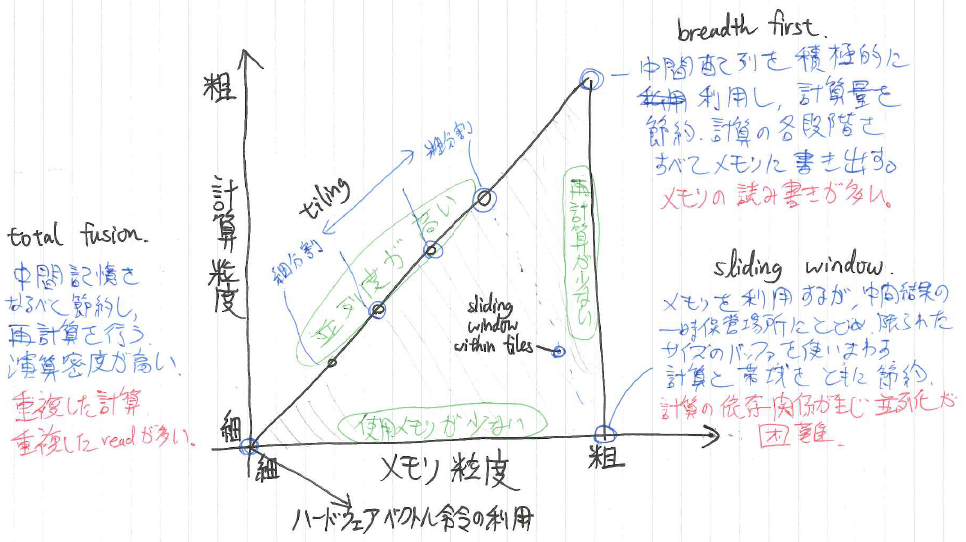
\includegraphics[width=10cm]{figure/doc/schedule-space.png}
\end{center}
\end{frame}


\begin{frame}\frametitle{Halideがサポートするプログラム変換の種類}
\begin{itemize}
  \item 分割:1..(M*N)までのループを1..Mと1..Nの二重ループに分割する
  \item 融合:1..Mと1..Nの2つのループを1つにまとめてしまう
  \item スレッド並列化:各添字を並列に計算
  \item アンロール:固定長のループを全部展開してループを消す
  \item ベクトル化:固定長のループをベクトル命令に置き換える
  \item タイル化:2次元のブロックを用意しそれを更新
  \item 入れ子ループの入れ替え
  \item 特殊化:条件変数が真の場合と偽の場合でループを分けループの中身を簡単化
\end{itemize}
\end{frame}

\begin{frame}[fragile]\frametitle{fma命令の生成}

例えば、{\tt .bc}ファイルを生成した上で、Bulldozer向けアセンブリを生成させることで、
fma(融合加乗算)命令を含むアセンブリを生成できる。
\begingroup
    \fontsize{8pt}{9pt}\selectfont
\begin{verbatim}
clang -O1 -march=bdver1 -ffp-contract=fast blur.bc -S
\end{verbatim}
\endgroup
\vspace{-1cm}


\end{frame}


\section{ベンチマーク}
\begin{frame}\frametitle{ベンチマーク環境}
\begin{center}
  \begin{tabular}{|c|c|}
    \hline
    マシン名 & armagnac0\\
    CPU & Bulldozer, 64 cores \\
    Memory & 256GB \\
    \hline
  \end{tabular}
\end{center}
\end{frame}


\begin{frame}[allowframebreaks]{参考文献}{}
  \bibliographystyle{apalike}
  \bibliography{bunken}
\end{frame}



% \begin{bibliography}
% 
% \bibitem[de~Saussure, 1995]{Saussure1995}
% de~Saussure, F. (1995).
% \newblock {\em Cours de Linguistique Grale}.
% \newblock Payot.
% 
% \bibitem[Labov, 1972]{Labov1972}
% Labov, W. (1972).
% \newblock {\em Sociolinguistic Patterns}.
% \newblock University of Pennsylvania Press, Philadelphia.
% 
% \end{bibliography}








\section*{リサイクルボックス}




\subsection{}
\begin{frame}\frametitle{}
\begin{eqnarray}
\end{eqnarray}
\end{frame}


\begin{frame}[fragile]\frametitle{}
\begingroup
    \fontsize{8pt}{9pt}\selectfont
\begin{verbatim}
subroutine kernel__velderiv()
\end{verbatim}
\endgroup
\vspace{-1cm}
\end{frame}




\end{document}

